\subsubsection{Data Type}
Based on our data, we observed that the largest effect stemmed from the data type being shared in a scenario. We present various statistical models in section \ref{sec:regression} to support this conclusion. The 10 most and 10 least concerning data types can be seen in Table \ref{top10}. 

Regardless of the data recipient or the device, participants were most concerned about photos and videos, especially if they contained embarrassing content, nudity, or financial information. As seen in Table \ref{top10-table}, photos and videos accounted for 5 of the top 10 concerns, {\color {red} and are unanimously considered to be concerning}. Information that could be used to impersonate someone (e.g., usernames/passwords for websites) or invade privacy (photos of someone at home) were also among the most concerning data types. 

Also regardless of the other factors, the least concerning data types mostly consisted of information that could be observed through observations of public behavior, such as demographic information (e.g., age, gender, language spoken). {\color {red} As seen in Table \ref{top10-table}, participants had distributed opinions on how risky this information was to be shared. A possibility is that people rated these as unconcerning because of unfamiliarity in what applications would use this data for, or because there does not seem to be any immediate financial, social, or physical consequences from having this information shared.}

{\color {red} talk about the variance of the data types here, referring to the table in the appendix. Which were the highest in variance? Which were the unanimous? Which one had a spread? Were there any that were specifically polarized? J has yet to give me the table for this so I can talk about it. But the most unanimous ones seemed to be the highest-concerning ones, whereas the least concerning ones were more distributed. There are not any which are unanimously considered medium risk or to be not risky.}

\begin{table}[t]
\begin{center}
\small
\begin{tabular}{| r | l | r | l |c |}
\hline
Rank & Data & VUR & sd & Distribution \\
\hline
1 & a video of you unclothed & 95.97\% & number & 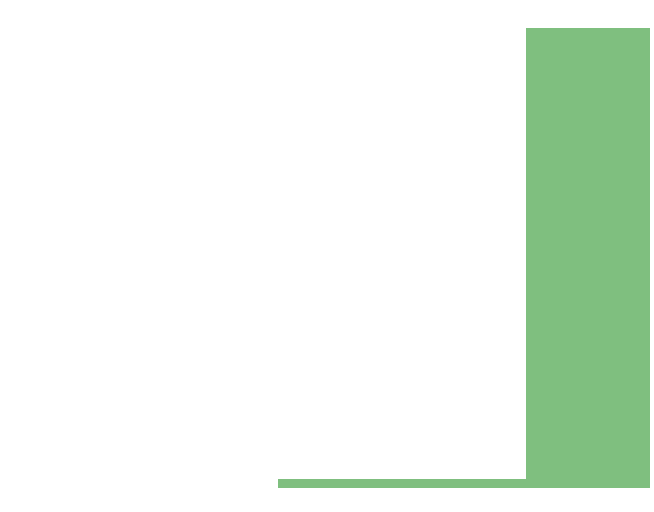
\includegraphics[width = 2cm, height = 0.5cm]{tex-inputs/data10/tookavideoofyouunclothedcombined} \\
2 & bank account information & 95.91\% & number & 
\includegraphics[width = 2cm, height = 0.5cm]{tex-inputs/data10/learnedyourbankaccountinformationcombined}  \\
3 & social security number & 94.84\% & number & 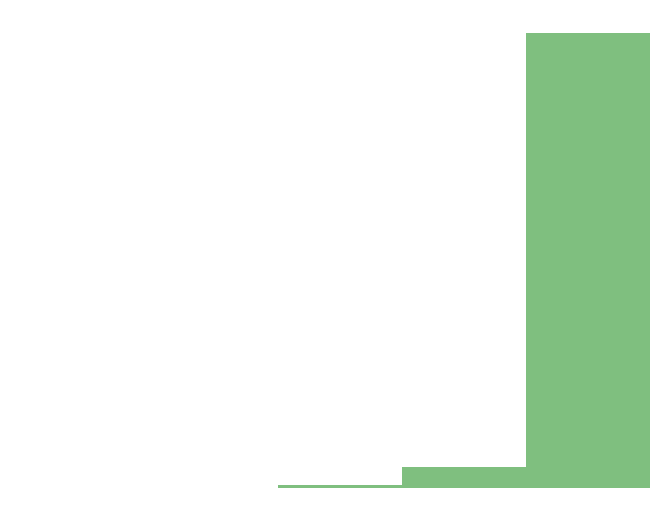
\includegraphics[width = 2cm, height = 0.5cm]{tex-inputs/data10/learnedyoursocialsecuritynumbercombined}\\
4 & video of you entering in your PIN & 92.67\% & number & 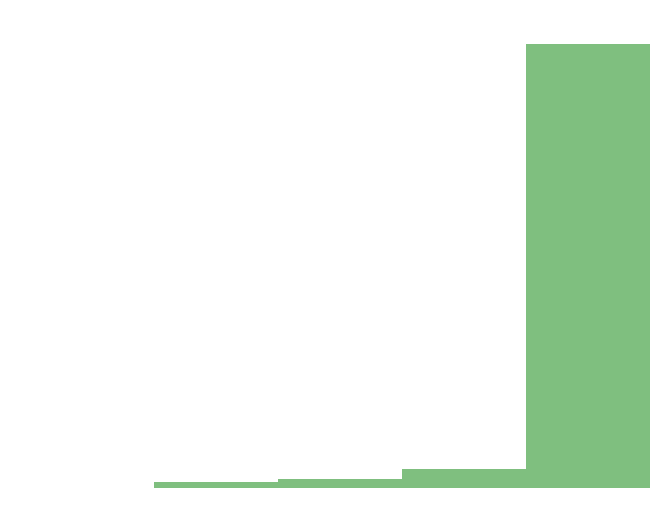
\includegraphics[width = 2cm, height = 0.5cm]{tex-inputs/data10/tookavideoofyouenteringinyourPINatanATMcombined}\\
5 & a photo of you unclothed & 92.59\% & number & 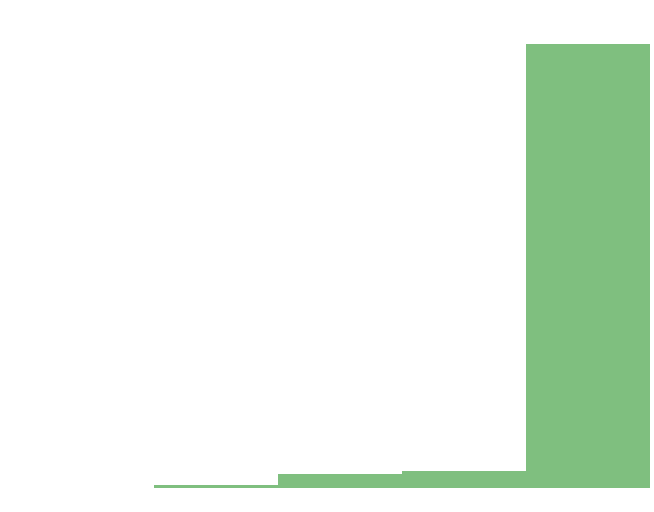
\includegraphics[width = 2cm, height = 0.5cm]{tex-inputs/data10/tookaphotoofyouunclothedcombined}\\
6 & an incriminating/embarrassing photo of you & 91.39\% & number & 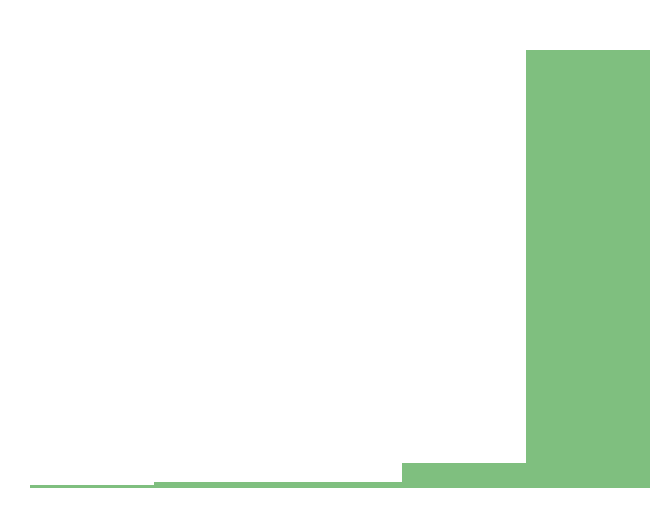
\includegraphics[width = 2cm, height = 0.5cm]{tex-inputs/data10/tookanincriminatingphotoofyoudoingsomethingembarrassingcombined}\\
7 & username and password for websites & 89.55\% & number & 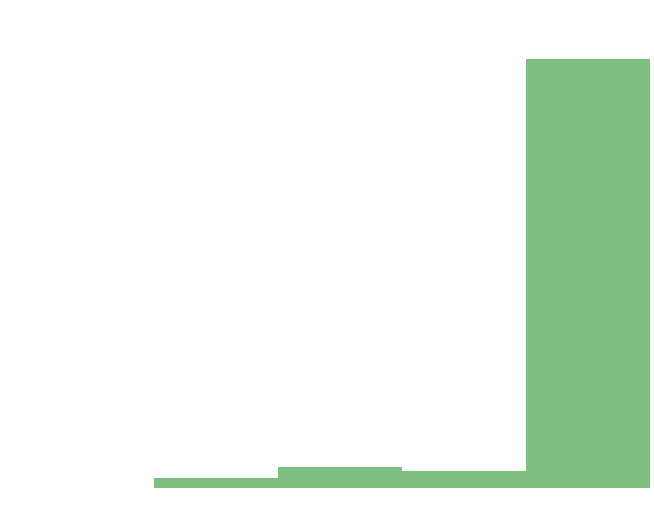
\includegraphics[width = 2cm, height = 0.5cm]{tex-inputs/data10/learnedyourusernameandpasswordforwebsitescombined}\\
8 & credit card information & 88.98\% & number & 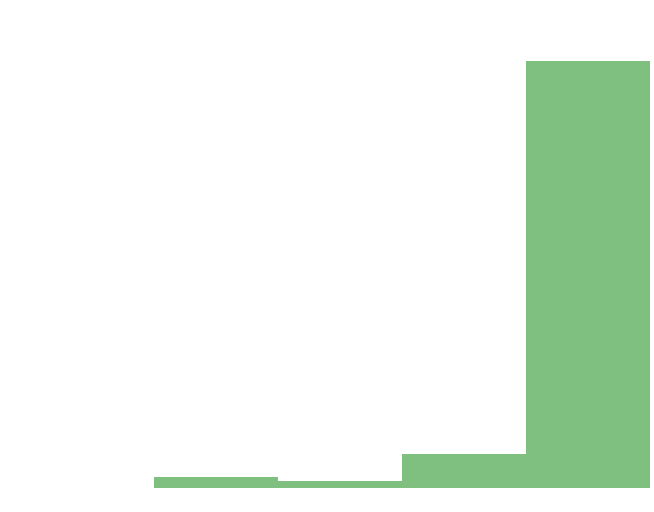
\includegraphics[width = 2cm, height = 0.5cm]{tex-inputs/data10/learnedyourcreditcardinformationcombined}\\
9 & an incriminating/embarrassing video of you & 88.41\% & number & 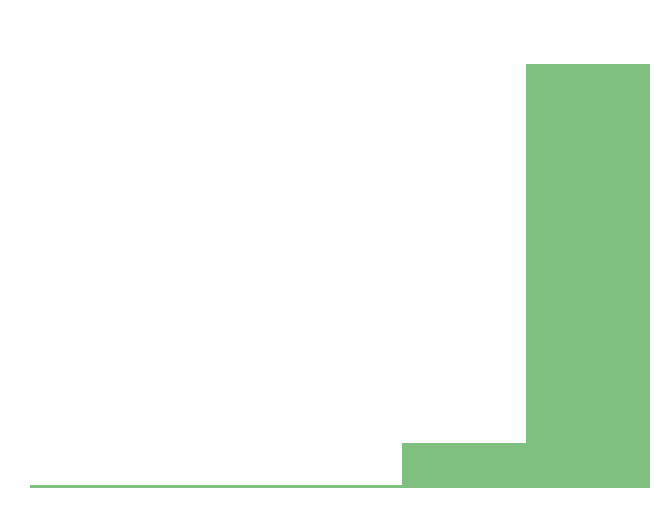
\includegraphics[width = 2cm, height = 0.5cm]{tex-inputs/data10/tookanincriminatingvideoofyoudoingsomethingembarrassingcombined}\\
10 & a random (inward-facing) photo you at home & 87.50\% & number & 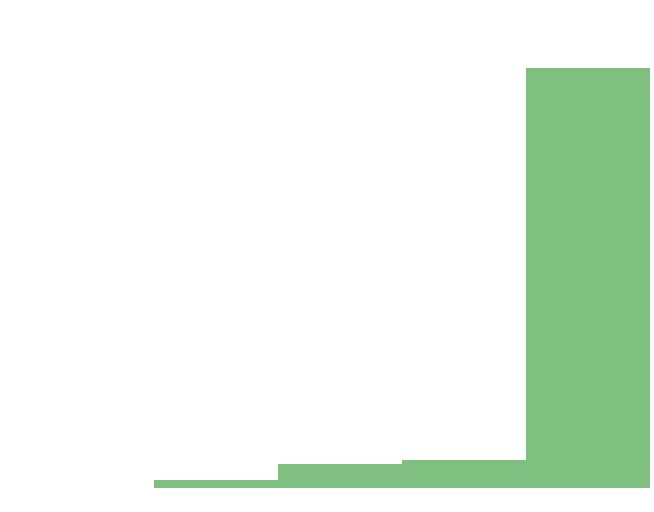
\includegraphics[width = 2cm, height = 0.5cm]{tex-inputs/data10/tookphotosofyou(withaninward-facingcamera)athomecombined}\\
 & \vdots & \\
64 & eye movement patterns (for eye tracking) & 40.51\%& number & 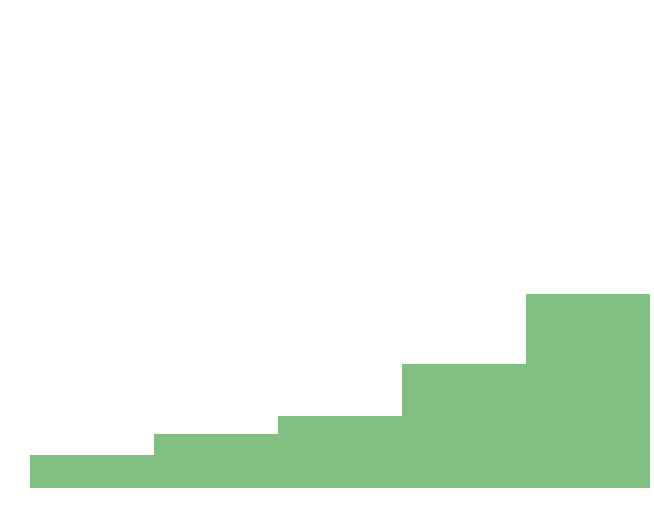
\includegraphics[width = 2cm, height = 0.5cm]{tex-inputs/data10/scannedyoureyetolearnyoureyepatterns(foreyetracking)combined} \\
65 & when and how much you exercise  & 38.66\% & number & 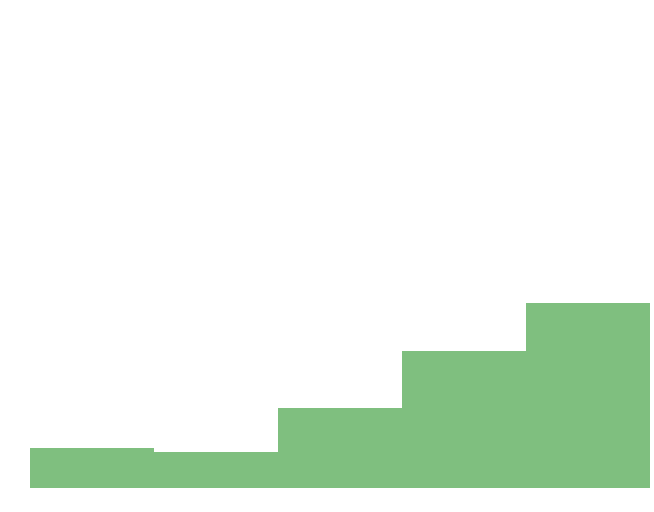
\includegraphics[width = 2cm, height = 0.5cm]{tex-inputs/data10/learnedwhenhowandhowmuchyouexercisecombined}\\
66 & when you are happy or having fun  & 34.75\% & number & 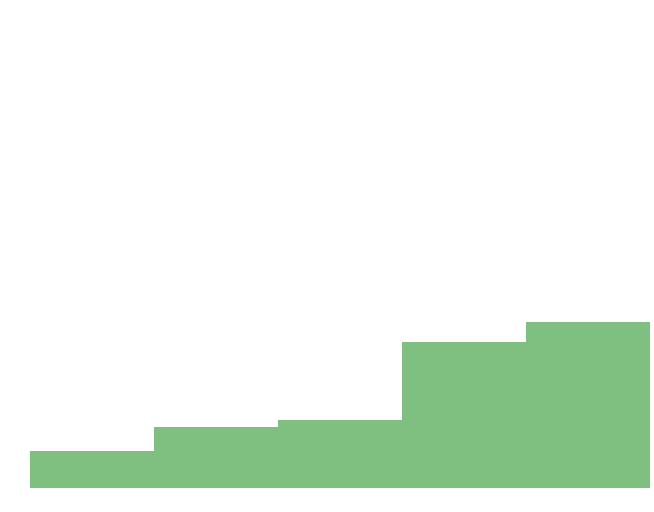
\includegraphics[width = 2cm, height = 0.5cm]{tex-inputs/data10/learnedwhenyouwerehappyorhavingfuncombined}\\
67 & which television shows you watch & 30.20\% & number & 
\includegraphics[width = 2cm, height = 0.5cm]{tex-inputs/data10/learnedwhattelevisionshowsyouwatchcombined}\\
68 & when you are busy or interruptible  & 29.50\% & number & 
\includegraphics[width = 2cm, height = 0.5cm]{tex-inputs/data10/learnedwhenyouarebusyorinterruptiblecombined}\\
69 & music from your device  & 28.06\% & number & 
\includegraphics[width = 2cm, height = 0.5cm]{tex-inputs/data10/copiedanduploadedmusicfromyourdevicecombined}\\
70 & your heart rate & 27.50\% & number & 
\includegraphics[width = 2cm, height = 0.5cm]{tex-inputs/data10/learnedyourheartratecombined} \\
71 & your age & 24.29\% & number & 
\includegraphics[width = 2cm, height = 0.5cm]{tex-inputs/data10/learnedyouragecombined}\\
72 & the language you speak & 15.86\% & number & 
\includegraphics[width = 2cm, height = 0.5cm]{tex-inputs/data10/learnedthelanguageyouwerespeakingcombined}\\
73 & your gender & 15.00\% & number & 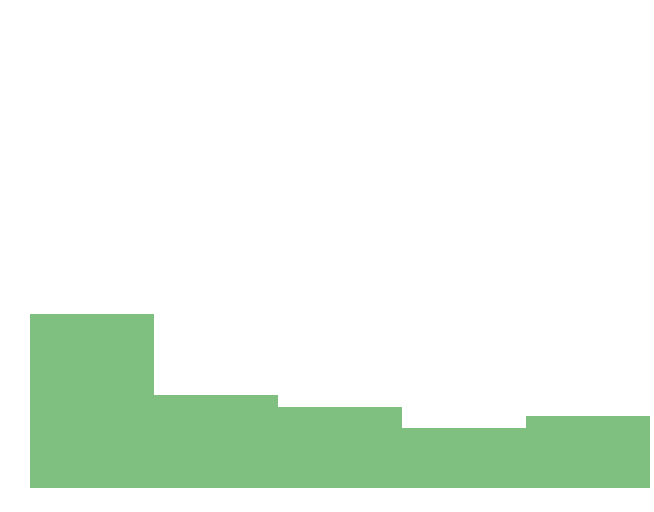
\includegraphics[width = 2cm, height = 0.5cm]{tex-inputs/data10/learnedyourgendercombined}\\ 
\hline
\end{tabular}
\caption{The 10 most and least upsetting data types, across all recipients.}
\label{top10-table}
\end{center}
\end{table}

The data types the we examined span several existing and future use cases. However, we do not necessarily believe they are comprehensive or cover all possible future use cases for how wearable devices might capture personal data. As such, we decided to code each data type in terms of both the capture medium (e.g., video, audio, text, etc.) and the type of risk to which it might expose the user. The purpose of this was to examine {\it why} participants viewed certain data types as more or less risky than others so that we can then generalize our results to other data types that were not covered by this particular survey instrument. To this end, two researchers agreed on a codebook and then independently coded each of the 72 data types\footnote{We excluded the data types that did not feature a data recipient.} in terms of the medium used for collection and in terms of the type of risk posed to the user. The mediums fell into six possible categories:

\begin{enumerate}
\item Photo
\item Video
\item Audio
\item Behavioral Information
\item Biometric Information
\item Demographic Information
\end{enumerate}

The associated risks with each data type fell into the following five categories:

\begin{enumerate}
\item {\bf Financial:} The risk involves the loss of money or property.
\item {\bf Image:} The risk involves loss of control over one's self-image (e.g., publicizing something embarrassing).
\item {\bf Medical:} The risk involves disclosure of medical information.
\item {\bf Physical:} The risk involves physical harm to the user.
\item {\bf Relationships:} The risk involves damage to the user's inter-personal relationships.
\end{enumerate}

Upon independently coding each data type along these two axes, the researchers met to resolve any disagreements, such that the resulting codings reflected unanimity. Prior to this resolution, they agree on 83\% of the codings. Cohen's $\kappa$ was 0.75 for the risks and 0.81 for the mediums, both indicating ``excellent'' agreement~\cite{Fleiss2003}.

%A statistical analysis regarding the significance and confidence of <data> types with respect to all 72 was not performed due to the space constraints of the paper. We do consider all <data> categories in our statistical model, which provides an analysis of what factors had contributed to the perceived severity of a particular situation. 









